\documentclass{beamer}
\usepackage{graphicx} % Required for inserting images
\usepackage{booktabs}
\usepackage{hyperref}
\hypersetup{
    urlcolor=cyan,
    pdftitle={V0 Projet},
    pdfpagemode=FullScreen,
    }
\usepackage{float}
\usepackage{listings}
\usepackage{amsmath}
\usepackage{array}
\usepackage[french]{babel}
\usetheme{CambridgeUS}
\newcommand\Includegraphics[2][]{%
  \raisebox{-.5\dimexpr\height-\ht\strutbox+\dp\strutbox}{\includegraphics[#1]{#2}}}

\title{BDR Thermea: Modèle 3D d'une turbine toroïdale}
\author{Sacha Alidadi Heran}
\date{Novembre 2023}

\begin{document}

\maketitle

\begin{frame}{Contexte et objectif}
    \begin{itemize}
        \item Nous voulons réduire le bruit de l'unité extérieure d'une pompe à chaleur
        \item Pour ça nous allons tester un nouveau modèle de turbine en forme toroïdale
        \item Ce modèle a fait ces preuves pour des hélices de drone, mais doit être testé
        \item Objectif: Créer un modèle de turbine toroïdal 3D
    \end{itemize}
\end{frame}

\begin{frame}{Visualisation}
    \begin{columns}[T]
        \hfill
        \begin{column}{.32\textwidth}
            \hspace{2mm}\Includegraphics[height=0.6\textheight]{images/Curve1D.png} \hspace{2mm}\\
        \end{column}
        \hfill
        \begin{column}{.32\textwidth}
            \begin{itemize}
                \item Nous avons pu générer la courbe guide d'une hélice grâce au papier suivant \href{http://www.ship-research.com/cn/article/doi/10.19693/j.issn.1673-3185.03419}{[1]}
            \end{itemize}
        \end{column}
        \hfill
    \end{columns}
\end{frame}

\begin{frame}{Roadmap}
    \begin{figure}
        \centering
        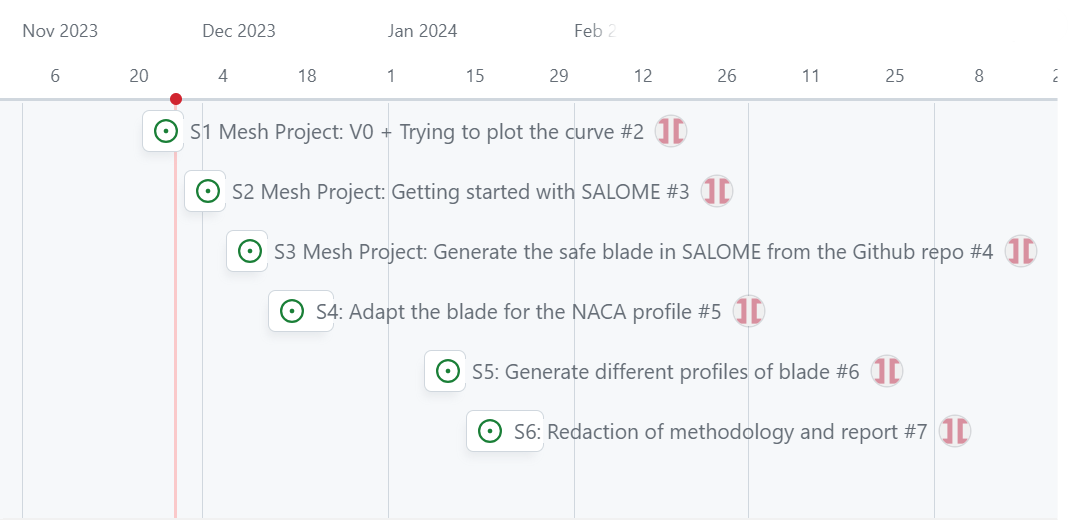
\includegraphics[scale=0.5]{images/RoadmapV0.png}
        \caption{Roadmap du projet}
        \label{fig:Roadmap}
    \end{figure}
\end{frame}

\begin{frame}{Bibliographie}
    \begin{itemize}
        \item Mathematical expression method for geometric shape of toroidal propeller, YE Liyu, WANG Chao, SUN Cong, GUO Chunyu, 2023 \href{http://www.ship-research.com/cn/article/doi/10.19693/j.issn.1673-3185.03419}{[1]}
        \item Toroidal propeller generator \href{https://github.com/RaulBejarano/Ultimate-Toroidal-Propeller-Generator}{[2]}
        \item Toroidal propeller MIT \href{https://www.ll.mit.edu/sites/default/files/other/doc/2023-02/TVO_Technology_Highlight_41_Toroidal_Propeller.pdf}{[3]}
        \item P. RATHOA - Private Communication [4]
    \end{itemize}
\end{frame}

\end{document}